%-----------------------------------------------------------------------------
%
%               Template for sigplanconf LaTeX Class
%
% Name:         sigplanconf-template.tex
%
% Purpose:      A template for sigplanconf.cls, which is a LaTeX 2e class
%               file for SIGPLAN conference proceedings.
%
% Guide:        Refer to "Author's Guide to the ACM SIGPLAN Class,"
%               sigplanconf-guide.pdf
%
% Author:       Paul C. Anagnostopoulos
%               Windfall Software
%               978 371-2316
%               paul@windfall.com
%
% Created:      15 February 2005
% Modified:    12 October 2016 by Kent D. Lee for 
%                    Luther CS Department Requirements. 
%
%-----------------------------------------------------------------------------


\documentclass[10pt]{luthercs}
\usepackage{listings}
\usepackage{graphicx}
% The following \documentclass options may be useful:

% preprint      Remove this option only once the paper is in final form.
% 10pt          To set in 10-point type instead of 9-point.
% 11pt          To set in 11-point type instead of 9-point.
% numbers       To obtain numeric citation style instead of author/year.

\usepackage{amsmath}

\newcommand{\cL}{{\cal L}}

\begin{document}

\special{papersize=8.5in,11in}
\setlength{\pdfpageheight}{\paperheight}
\setlength{\pdfpagewidth}{\paperwidth}

\title{Type Inference for Language Prototyping}
%\subtitle{A }

\authorinfo{Kent D. Lee}
           {Luther College}
           {kentdlee@luther.edu}
%\authorinfo{Name2\and Name3}
%          {Affiliation2/3}
%           {Email2/3}

\maketitle

\begin{abstract}
This paper provides an overview of a framework for prototyping programming languages while providing an in-depth description of type inference for a subset of Standard ML, implemented in Prolog. As part of this research, type inference rules for Standard ML were developed along with an implementation utilizing the full unification power of Prolog. The paper details the techniques used to implement type inference in Prolog and describes how the larger framework may be applied to other language prototyping.  

\end{abstract}

\section{Introduction}

Prototyping a language often leads to discovery. The prototyping framework presented in this paper consists of a virtual machine, a compiler from a sample source language to the virtual machine, and a type inference system. The type inference system is covered in detail in this paper. Another paper \cite{Lee15} provides a more detailed overview of the entire framework.

Prototyping a language is easier when compiling to a virtual machine. Python is a programming language that supports imperative, object-oriented, and functional programming. Internally, Python is compiled to a virtual machine before it is interpreted. The Python virtual machine is seen as an implementation detail of Python and is not guaranteed to remain stable like externalized virtual machines. The Python virtual machine is not an externalized interface to which other languages could be targeted. 

While the Java Virtual Machine is an externalized virtual machine, it is not suitable as a target language in many cases. The Java Virtual Machine does not directly support nested functions and static scope. Nested inner classes are supported, but not in the same way that nested functions are supported in many functional languages. Supporting nested functions and static scope within the JVM would require support from a set of classes. In other words, a supporting run-time system would be required. An externalized Python virtual machine would be better suited as a target for languages with nested functions and scope since no run-time system is needed, thus simplifying the generated code.

\begin{figure}[htbp]
\hbox{\hspace{0.5in}
\begin{lstlisting}[language=ML, numbers=left,numberstyle=\tiny]
let fun f(x,y) = 
  let fun g(x,y) = 
    if x < 1 then y else f(y-1,x)
  in
    g(x,y)
  end
in
  println(f(5,12))
end
\end{lstlisting}}
\caption{A Standard ML Program}
\label{mlprog}
\end{figure}

\begin{figure}[htbp]
\hbox{\hspace{0.5in}
\begin{lstlisting}[language=Python, numbers=left,numberstyle=\tiny]
import disassembler
def f(x,y):
  def g(x,y):
    if x < 1:
      return y
    else:
      return f(y-1,x)
  return g(x,y)
def main():
  print(f(5,12)) 
main()
#disassembler.disassemble(f)
#disassembler.disassemble(main)
\end{lstlisting}}
\caption{A Python Program}
\label{pyprog}
\end{figure}

CoCo is an externalized Python Virtual Machine. CoCo was built by reverse engineering the Python virtual machine. It is written in C++, using Object-Oriented design principles like inheritance, information hiding, and polymorphism. It is easily extensible for language prototyping. And, it has a stable interface that will remain backwards compatible. In addition, CoCo includes a disassembler of Python 3.2 programs that can be used to discover correct code for implementing various language features. For instance, consider the ML program in figure~\ref{mlprog} (liberty was taken with the use of println - so not quite ML). A similar program can be written in Python, as shown in figure~\ref{pyprog}, to discover how to implement the ML program using the CoCo virtual machine. By commenting out the call to the {\em main} function and uncommenting the calls to a CoCo disassembler module, the Python program can be disassembled to discover its CoCo implementation. The CoCo version of the programs presented in figures~\ref{mlprog} and \ref{pyprog} is presented in appendix~\ref{cocoprog}. 

\begin{figure}[htbp]
\hbox{\hspace{0.5in}
\begin{lstlisting}[language=ML, numbers=left,numberstyle=\tiny]
let val x = 6
in 
  println(x+1)
end
\end{lstlisting}}
\caption{A Static Binding Example}
\label{mlprog2}
\end{figure}

\begin{figure}[htbp]
\hbox{\hspace{0.5in}
\begin{lstlisting}[language=ML, numbers=left,numberstyle=\tiny]
let val x = ref 6
in 
  println(!x+1)
end
\end{lstlisting}}
\caption{A Reference Example}
\label{mlprog3}
\end{figure}

Of course, not every program is going to have a direct counter-part in Python. But the disassembler can be used to discover many code generation {\em secrets} of Python to quickly familiarize the researcher with the virtual machine. Consider the ML program presented in figure~\ref{mlprog2}. Implementing this in CoCo requires the use of a variable to hold the value of {\em x}. There is no concept of static bindings in CoCo (like Python).  This means the generated CoCo code for figures~\ref{mlprog2} and \ref{mlprog3} are identical leaving room for a third version of this program in figure~\ref{mlprog4} which is not a valid ML program and yet compiles and runs successfully on the CoCo virtual machine. There are at least a couple of type errors in the program of figure~\ref{mlprog4} depending on how you go about fixing it. The variable {\em x} might be declared as a reference on line 1 which means that the dereferencing of {\em x} on lines 3 and 4 should be rewritten as {\em !x}. 
 

\begin{figure}[htbp]
\hbox{\hspace{0.5in}
\begin{lstlisting}[language=ML, numbers=left,numberstyle=\tiny]
let val x = 6
in 
  x := x + 1;
  println(x+1)
end
\end{lstlisting}}
\caption{An Invalid ML Program}
\label{mlprog4}
\end{figure}

Type inference or type checking is clearly an important part of any programming language, whether the type checking is done statically before run-time, or dynamically at run-time. 

\begin{figure}[htbp]
\centering
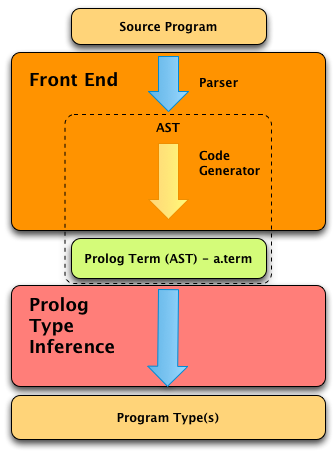
\includegraphics[width=3in]{hybrid.png}
\caption{Overview of the Framework}
\label{hybrid}
\end{figure}

\section{Mapping from Source to AST to Type}

Implementing type inference within the prototyping framework presented here first entails mapping a program into its abstract syntax. Then the type inference system maps from the abstract syntax tree (i.e. AST) into its type as depicted in figure~\ref{hybrid}. Abstract syntax and types must both be defined.  The abstract syntax of the {\em Small}  language is given in appendix~\ref{astdef}. 

Strings, integers, characters, and booleans are supported as primitive data. Small, like Standard ML, has a core language which the abstract syntax represents. Syntactic sugar is used to support language features like Curried functions, local bindings (i.e. let expressions) of more than one identifier, and anonymous functions. 

\begin{figure}[htbp]
\begin{lstlisting}[language=ML,numbers=left,numberstyle=\tiny]
datatype SmallType = 
        bool
      | int
      | str
      | exn
      | tuple of type list
      | listOf of type
      | fn of type * type
      | ref of type
      | typevar of string
      | typeerror
\end{lstlisting}
\caption{Small Types}
\label{smalltypes}
%\vspace{-.5in}
\end{figure}

The back end of the compiler writes to a file called {\em a.term} as depicted in figure~\ref{hybrid}, which is the Prolog term read by the type inference system part of the framework. The allowed syntax for the Prolog representation of the AST is given in appendix~\ref{astdef}. 

The type inference system maps the AST of a program into its type. The allowable types are given in figure~\ref{smalltypes}. As with many type systems, Small's type system is strict in {\em type errors} meaning that once a type error has been detected, the overall type of the expression is {\em typeerror}. Otherwise, we have the basic types, including exceptions, tuples, lists, functions, and references. The {\em typevar} is a Standard ML type inference variable used in representing polymorphic types as in Standard ML. Prolog does not require an explicit declaration of the allowable types. They are presented in figure~\ref{smalltypes} for reference only in the Standard ML datatype format. 

\section{The Type Environment}

The type environment is represented as $\varepsilon$ in the type inference rules of appendix~\ref{infrules}. The environment includes the types for built-in functions of the {\em Small} language. The infix operators of the language are also represented as functions in the abstract syntax and in the environment to increase uniformity and reduce the amount of code in the type checker. A complete description of the type environment can be found in \cite{leepl}. Part of the environment is given in figure~\ref{typeenv}.

\begin{figure}[htbp]
\begin{lstlisting}[language=Prolog,numbers=left,numberstyle=\tiny]
typecheckProgram(Expression,Type) :- 
  typecheckExp(
    [('Exception',fn(typevar(a),exn)),
     ('raise',fn(exn,typevar(a))),
     ('andalso',
      fn(tuple([bool,bool]),bool)),
     ('orelse',
      fn(tuple([bool,bool]),bool)),
     ('=', 
      fn(tuple([typevar(a),typevar(a)]),
       bool)),
     ('<', 
      fn(tuple([typevar(a),typevar(a)]),
       bool)),
     (@,
      fn(tuple([listOf(typevar(a)),
                 listOf(typevar(a))]),
      listOf(typevar(a)))),
     ('input',fn(str,str)),
     ('explode',fn(str,listOf(str))),
     ('implode',fn(listOf(str),str)),
     ('println',
      fn(typevar(a),tuple([]))),
     ('type',fn(typevar(a), str)),
     (+,fn(tuple([int,int]),int)),
     (-,fn(tuple([int,int]),int)),
     (*,fn(tuple([int,int]),int)),
     ...
     ('div',fn(tuple([int,int]),int))],
     Expression,Type).
\end{lstlisting}
\caption{The (partial) Type Environment}
\label{typeenv}
%\vspace{-.5in}
\end{figure}

Type inference rules map from the AST definition of a program to its type. This mapping, from AST to its type dictates that several Prolog predicates be written, including {\em typeCheckExp}, {\em typeCheckMatch}, {\em typeCheckPat}, and {\em typecheckDec}, all corresponding to the various abstract syntax node types. There are also a number of supporting predicates that are written for these main predicates. 

Type checking a program in the prototyping framework starts by setting up the environment and calling the {\em typeCheckExp} Prolog predicate to instantiate a type given a program (i.e. a {\em Small} expression). The implementation of {\em typeCheckExp} is dictated by the type inference rules presented in the next sections and appendix~\ref{infrules}.


\section{Type Inference}

Type inference rules are presented in the standard format of antecedents over conclusions. A type environment is represented as $\varepsilon$ as described in the last section. The complete set of type inference rules for the {\em Small} language are presented in appendix~\ref{infrules} and can also be found in \cite{leepl}. 

Type checking a simple constant value does not require the type environment, but it is included for consistency. For instance, consider the {\em BoolCon} rule. The environment is not needed because the constant is already labeled with its type. The Prolog code that corresponds to this inference rule is given in figure~\ref{boolcon}.

\begin{description}
\item[{\textbf{BoolCon}}] \begin{gather}
\begin{split}\frac{}{\varepsilon\vdash bool(v) : bool}\end{split}\notag
\end{gather}
\end{description}


\begin{figure}[htbp]
\begin{lstlisting}[language=Prolog]
typecheckExp(_,bool(_),bool):-!.
\end{lstlisting}
\caption{BoolCon Prolog Definition}
\label{boolcon}
%\vspace{-.5in}
\end{figure}

The cut operator (i.e. \verb+!+) used in figure~\ref{boolcon} is useful in this code. Without it, type checking a program that contained a boolean followed by another expression that could not be properly type checked due to some error in the coding of an inference rule or some unimplemented part of the type checking might undo the match of the boolean value in its attempt to backtrack and find another way to correctly type check the given expression. 

For example, consider type checking this expression. 

\begin{lstlisting}[language=Prolog]
typecheckExp(Env,apply(id('='),
  tuple([bool('true'),E2])))
\end{lstlisting}

\noindent Assume that type checking expression {\em E2} contains an error. Prolog would fail to find a way to satisfy the predicate for {\em typeCheckExp(Env, E2, T)} and then would backtrack to the {\em BoolCon} rule implementation, undo that unification, and then look for a further unifiable term, finding it at the end of the {\em typeCheckExp} code found in figure~\ref{typecheckcatchall}. Unifying with the code in figure~\ref{typecheckcatchall} it would print that {\em bool} is an unknown expression. 

\begin{figure}[htbp]
\begin{lstlisting}[language=Prolog]
typecheckExp(_,Exp,_) :- 
  print('Error: Unknown expression '), 
  print(Exp),
  throw(error('unknown expression')), !.
\end{lstlisting}
\caption{typeCheckExp Catch-All}
\label{typecheckcatchall}
%\vspace{-.5in}
\end{figure}

This sort of problem does not routinely occur, but debugging these problems is easier if the cut operator is applied to limit any unwanted backtracking. 

Verifying that all elements of a list constant are homogenous is one instance where Prolog's unification algorithm works exactly as desired. The {\em ListCon} rule requires all elements of a list constant have the same type.

\begin{description}
\item[{\textbf{ListCon}}] \begin{gather}
\begin{split}& \forall i~~1\leq i \leq n, n \geq 0\\
& \frac{\varepsilon\vdash e_i:\alpha}{\varepsilon\vdash [e_1,e_2,...,e_n] : \alpha~~list}\end{split}\notag
\end{gather}
\end{description}

Type checking a list constant requires a supporting predicate to call {\em typeCheckExp} on each of the elements of the list. Of course each element of the list must have the same type. The subtle code in this example is the first case of the {\em typecheckList} predicate. If the list is empty (i.e. \verb+[]+), then the type of the list is $\alpha~list$ where $\alpha$ is a Prolog variable that results from the use of the underscore in this definition. 

\begin{figure}[htbp]
\begin{lstlisting}[language=Prolog]
typecheckList(_,[],_) :- !.
typecheckList(Env,[H|T],A) :- 
  typecheckExp(Env,H,A), 
  typecheckList(Env,T,A), !.
typecheckExp(Env,listcon(L),listOf(T)):- 
  typecheckList(Env,L,T), !.
\end{lstlisting}
\caption{List Type Checking}
\label{listcon}
%\vspace{-.5in}
\end{figure}

There are two extensions to typical type inference rules that are used in the definition of the {\em Small} type inference rules. Inferring the type of a declaration produces a new type environment. This is indicated in rules like the {\em FunDecs} rule where the environment described to the right of the $\Rightarrow$ is yielded when successfully applying the rule to a program. These yielded environments are further applied to rules through the use of the $\oplus$ operator as used in the {\em Matches} or {\em FunDecs} rules, for instance. 

\begin{description}
\item[{\textbf{ConsPat}}] \begin{gather}
\begin{split}\frac{pat_1:\alpha\Rightarrow  \varepsilon_{pat_1},~~pat_2:\alpha~list\Rightarrow \varepsilon_{pat_2}}
     {pat_1::pat_2 : \alpha~list\Rightarrow \varepsilon_{pat_1}+\varepsilon_{pat_2}}\end{split}\notag
\end{gather}
\end{description}


\begin{description}
\item[{\textbf{TuplePat}}] \begin{gather}
\begin{split}&  \forall i~1 \leq i \leq n, n \geq 0\\
& \frac{pat_i : \alpha_i \Rightarrow \varepsilon_{pat_i}}
       {(pat_1,pat_2,...,pat_n): \times_{i=1}^{n}\alpha_i\Rightarrow \sum^{n}_{i=1}\varepsilon_{pat_i}}\end{split}\notag
\end{gather}
\end{description}

While the $\oplus$ operator indicates a possibly overlapping concatenation of environments where the left environment takes precedence over similarly named types in the right environment, the $+$ operator and the $\Sigma$ operator are restricted to concatenating non-overlapping environments. When $+$ is used in an inference rule, the type environments on either side of the $+$ cannot overlap. For instance, consider the {\em TuplePat} rule. The pattern identifiers within a tuple pattern cannot have the same name. In the {\em ConsPat} rule the same identifiers cannot be used in the head or the tail pattern.

New environments are yielded while type checking declarations and patterns. These new environments are consulted while type checking expressions that contain identifiers.  This propogation of type environment information is shown explicitly in the type inference rules for {\em Small} through the use of the $\Rightarrow$, $\oplus$, $+$, and $\Sigma$ operators. 

\section{Polymorphic Types}

Standard ML supports polymorphic functions and values. So, figure~\ref{valuepoly} is a valid Standard ML and {\em Small} program. However, without a little work, the Prolog type variable bound to {\em x} will be instantiated to $int~list$ by the first expression and therefore will not unify with $string~list$ when type checking the second expression.

\begin{figure}[htbp]
\begin{lstlisting}[language=ML,numbers=left,numberstyle=\tiny]
let val x = []
in
  1::x;
  "hi"::x
end
\end{lstlisting}
\caption{Polymorphic Values}
\label{valuepoly}
%\vspace{-.5in}
\end{figure}

\begin{figure}[htbp]
\begin{lstlisting}[language=Prolog]
typecheckDec(Env,bindval(Pat,E),NewEnv):- 
  typecheckPat(Pat,ExpType,NewEnv), 
  typecheckExp(Env,E,ExpType), 
  closeExp(Pat,ExpType).
\end{lstlisting}
\caption{Closing Value Types}
\label{valdec}
%\vspace{-.5in}
\end{figure}

The example in figure~\ref{valuepoly} illustrates the need for closing and instantiating types within the Standard ML type inference system. A Prolog variable will unify with the first term applied to it. So, without further work, the type $\alpha$ unifies with $int$ in the first expression. This demonstrates that type variables must be distinct from Prolog variables and provides an understanding of the need for {\em typevar} types in figure~\ref{smalltypes}. The {\em ValDec} rule closes the type of {\em e}, resulting in converting any Prolog variables in the type of $\alpha$ into a type containing polymorphic {\em typevar} types as needed. The code in figure~\ref{valdec} is the Prolog implementation of this rule. 

\begin{description}
\item[{\textbf{ValDec}}] \begin{gather}
\begin{split}\frac{pat:\alpha\Rightarrow\varepsilon_{pat},~~\varepsilon\vdash e:close(\alpha)}{\varepsilon\vdash val~pat=e\Rightarrow\varepsilon_{pat}}\end{split}\notag
\end{gather}
\end{description}

\begin{description}
\item[{\textbf{FunApp}}] \begin{gather}
\begin{split}\frac{\varepsilon\vdash e_1 : \alpha\rightarrow\beta, ~~ \alpha'\rightarrow\beta':inst(\alpha\rightarrow\beta),~~ \varepsilon\vdash e_2 : \alpha'}
     {\varepsilon\vdash e_1 e_2 : \beta'}\end{split}\notag
\end{gather}
\end{description}

\begin{figure}[htbp]
\begin{lstlisting}[language=Prolog]
typecheckExp(Env,apply(Exp1,Exp2),ITT):- 
  typecheckExp(Env,Exp1,fn(FT,TT)), 
  typecheckExp(Env,Exp2,Exp2Type), 
  inst(Exp2Type,Exp2TypeInst),
  catch(inst(fn(FT,TT), 
    fn(Exp2TypeInst,ITT)),_, 
  printApplicationErrorMessage(
    Exp1,fn(FT,TT),Exp2,Exp2Type,ITT)),!.
\end{lstlisting}
\caption{Instantiating Types}
\label{funapp}
%\vspace{-.5in}
\end{figure}

When the polymorphic value is applied in an expression, its polymorphic type may be instantiated into a type containing Prolog variables that are suitable for unification once again. This is illustrated in the {\em FunApp} rule. The corresponding Prolog code is given in figure~\ref{funapp}. The Prolog predicate creates an instance of the argument type as {\em Exp2TypeInst}. This instantiated argument type must unify with the argument type of the function. If it does not, a function application error message is printed. Otherwise, the type {\em ITT} is the resulting type of the function application. Closing and instantiating polymorphic types is covered in the next section. 

\section{Close and Inst}

Two operations, {\em close} and {\em inst} are needed to go between polymorphic types containing ML type variables and those containing Prolog (i.e. unifiable) variables. 
The {\em inst} operation is pretty straightforward and is covered first. The {\em inst} predicate simply calls the {\em instanceOf} predicate.

\begin{figure}[htbp]
\begin{lstlisting}[language=Prolog,numbers=left,numberstyle=\tiny]
exists(Env,Id):- 
  member((Id,_),Env), !.
instanceOfList(Env,[],[],Env).
instanceOfList(Env,[H|T],[G|S],NEnv):- 
  instanceOf(Env,H,G,Env1), 
  instanceOfList(Env1,T,S,NEnv).
instanceOf(Env,A,A,Env):-var(A), !.
instanceOf(Env,A,A,Env):-simple(A), !. 
instanceOf(Env,fn(A,B), 
    fn(AInst,BInst),Env2):-  
  instanceOf(Env,A,AInst,Env1), 
  instanceOf(Env1,B,BInst,Env2), !.
instanceOf(Env,listOf(A),
    listOf(B),NEnv):- 
  instanceOf(Env,A,B,NEnv), !.
instanceOf(Env,ref(A),ref(B),NEnv):- 
  instanceOf(Env,A,B,NEnv), !. 
instanceOf(Env,tuple(L),tuple(M),NEnv):- 
  instanceOfList(Env,L,M,NEnv), !.
instanceOf(Env,typevar(A),B,Env):- 
  exists(Env,A), find(Env,A,B), !.
instanceOf(Env,
    typevar(A),B,[(A,B)|Env]):-!.
instanceOf(_,A,B,_):- 
  print('Type Error: Type '), 
  printType(B,_), 
  print(' is not an instance of '), 
  printType(A,_), nl, 
  throw(
    typeerror('type mismatch')), !.
inst(X,Y):-instanceOf([],X,Y,_).
\end{lstlisting}
\caption{The Inst Predicate}
\label{inst}
%\vspace{-.5in}
\end{figure}

Line 8 of figure~\ref{inst} handles any simple types like {\em int} and {\em bool} where the type is a simple atom. No need to write code for each individual primitive type in this case.

The real purpose of the {\em instanceOf} predicate is to remember the instantiation of all ML type variables and their Prolog counterparts. When a {\em typevar(a)} is found within a type expression, any other occurrences of {\em typevar(a)} within the type expression should be instantiated to the same Prolog type variable. That is the purpose of lines 20 and 21 in the {\em instanceOf} definition. 

If the Prolog interpreter attempts to satisfy the definition of {\em instanceOf} on lines 20-21 and fails, then it will backtrack and attempt to satisfy {\em instanceOf} using lines 22-23. It is here where the {\em typevar(a)} gets instantiated to the Prolog variable {\em B}. The {\em instanceOf} predicate also yields a new environment, adding the mapping of {\em typevar(a)} to {\em B} into the evironment so any further occurrences of {\em typevar(a)} may also be replaced with Prolog variable {\em B}. Notice that while {\em B} appears twice in lines 22-23, it is uninstantiated at this point and will unify with another type expression during type inference.

\begin{figure}[htbp]
\begin{lstlisting}[language=Prolog,numbers=left,numberstyle=\tiny]
closeFunTypes([]) :- !.
closeFunTypes([(Id,Type)|Tail]) :-
  closeFunTypes(Tail), print('val '), 
  print(Id), print(' = fn : '), 
  printType(Type,_), nl, !.
closeExp(Pat,Type) :-  
  print('val '), 
  printPat(Pat), print(' : '), 
  printType(Type,_), nl, !.
\end{lstlisting}
\caption{The Close Predicate}
\label{close}
%\vspace{-.5in}
\end{figure}

Closing a type is a bit more nuanced. A side-effect of closing a type is printing its type to the screen. Seeing the types of all named functions and values within an expression can be useful in some circumstances. So, closing a type and printing it to the screen happen at the same time. Because functions and values are printed slightly differently, there is a {\em closeFunTypes} predicate and a separate {\em closeExp} predicate. Both predicates call the {\em printType} predicate which does the actual closing of the type. 

Recall that closing a type means instantiating any Prolog variables to an ML {\em typevar} instance. This happens in the first four lines of figure~\ref{printtype}. Any Prolog variable will unify with the first term it encounters. When printing a type, a Prolog variable will unify with the first definition of {\em printTypeH}. Thus, the Prolog variable becomes instantiated to a {\em typevar}. 

The {\em printTypeH} also remembers any uninstantiated {\em typevar} variables it encounters by building a list of all uninstantiated typevars found in an expression. If a Prolog variable is instantiated in lines 1-4, the value to which it is instantiated, {\em typevar(A)} also contains an uninstantiated Prolog variable {\em A}. So, {\em printTypeH} is able to distinguish between an uninstantied Prolog variable on lines 1-4, and a previously instantiated {\em typevar} variable on lines 5-6. If the final program contains uninstantiated Prolog type variables, a warning message is printed that the uninstantiated types were instantiated to dummy type variables. For example, consider the trivial {\em Small} program of \verb+[]+. When this program is type checked, its resulting type is $\alpha~list$. The type inference system reports that $\alpha$ was instantiated to a dummy variable. 

The call to the {\em getNextVar} on lines 4-5 instantiates {\em A} to a unique {\em typevar} identifier after it was determined that {\em A} was uninstantiated previously. Notice that printType builds an environment of uninstantiated type variables, but does not ever use that environment. No environment is needed since the unclosed type contains Prolog variables and unification automatically converts all occurrences of an uninstantiated type to its instantiated counter-part at the same time. Prolog's unification mechanism makes it possible to close a type without the use of any extra environment. Effectively, the environment is maintained by Prolog in this case.

\begin{figure}[htbp]
\begin{lstlisting}[language=Prolog,numbers=left,numberstyle=\tiny]
printTypeH(Env,typevar(A),NewEnv):- 
  var(A), getNextVar(Env,A), 
  printTypeH([A|Env],
    typevar(A),NewEnv),!.
printTypeH(Env,typevar(A),[A|Env]):- 
  print(''''), print(A), !.
printTypeH(Env,tuple([]),Env):- 
  print(unit), !.
printTypeH(Env,tuple(L),NewEnv):-
  printTupleTypeH(Env,L,NewEnv), !. 
printTypeH(Env,listOf(A),NewEnv):-
  printSubTypeH(Env,A,NewEnv), 
  print(' list'),!.
printTypeH(Env,ref(A),NewEnv):- 
  printSubTypeH(Env,A,NewEnv), 
  print(' ref'),!.
printTypeH(Env,fn(A,B),Env2):- 
  var(A), printSubTypeH(Env,A,Env1), 
  print(' -> '), 
  printTypeH(Env1,B,Env2),!.
printTypeH(Env,fn(tuple(L),B),NewEnv):- 
  printTypeH(Env,tuple(L),Env1), 
  print(' -> '), 
  printTypeH(Env1,B,NewEnv),!.
printTypeH(Env,fn(A,B),Env2):- 
  printSubTypeH(Env,A,Env1), 
  print(' -> '), 
  printTypeH(Env1,B,Env2), !.
printTypeH(Env,typeerror,Env):- 
  print(typeerror), !.
printTypeH(Env,T,Env):- 
  simple(T), print(T), !. 
printTypeH(Env,T,Env):- 
  print('Error: unknown type '), 
  print(T), 
  throw(typeerror('unknown type')),!.
printType(T,TypeVars):- 
  printTypeH([],T,TypeVars).
\end{lstlisting}
\caption{The PrintType Predicate}
\label{printtype}
%\vspace{-.5in}
\end{figure}

\section{Mutually Recursive Functions}

Type checking mutually recursive functions creates some special challenges. When functions are mutually recursive their types may also be mutually dependent on each other. This is another instance where the unification algorithm is useful. The {\em FunDecs} rule is fairly complicated to read. It specifies that to type check a series of mutually recursive functions, each function is first assigned a type $\alpha_i \rightarrow \beta_i$. The types $\alpha_i$ and $\beta_i$ are Prolog variables initially. 

\begin{description}
\item[{\textbf{FunDecs}}] \begin{gather}
\frac{\begin{split}&  \forall i~1 \leq i \leq n, \forall j~1 < j \leq n,~~n \geq 1,\\
& [id_1\mapsto\alpha_1\rightarrow\beta_1~\{,~id_j\mapsto\alpha_j\rightarrow\beta_j\}]\oplus\varepsilon\vdash \\ & ~~~~id_i~matches_i:\alpha_i\rightarrow\beta_i\end{split}}{\begin{split} & \varepsilon\vdash f\!un~id_1~matches_1~\{and~id_j~matches_j\}\Rightarrow \\ & ~~~~[id_1\mapsto close(\alpha_1\rightarrow\beta_1)~\{,~id_j\mapsto close(\alpha_j\rightarrow\beta_j)\}]\end{split}}\notag
\end{gather}
\end{description}

To implement this rule, an auxiliary predicate called {\em gatherFuns} is used to collect the list of mutually recursive functions, assign each of them an $\alpha_i \rightarrow \beta_i$ type, and bind each of the function identifiers to their types in the type environment. Notice that the {\em typecheckFun} predicate does not yield a type. This is because the types of each of the potentially mutually recursive functions is further specified in the environment as function applications are type checked. Each time a function is applied, either its $\alpha_i$ or $\beta_i$ type is further specified, or both. However, the {\em FunApp} rule creates a new instance of a type each time the function is applied. This would hinder the further narrowing of the types in the mutually recursive functions except for line 7 of figure~\ref{inst} which specifies that creating an instance of a type which is already a Prolog variable leaves the Prolog variable {\em as-is}, leaving the original Prolog variable in place. The {\em inst} operation only creates instances of ML type variables. Prolog type variables are left {\em as-is}. 

\begin{figure}[htbp]
\begin{lstlisting}[language=Prolog,numbers=left,numberstyle=\tiny]
gatherFuns([],[]):-!.
gatherFuns([funmatch(Id,_)|Tail],
  [(Id,fn(_,_))|FEnv]):- 
    gatherFuns(Tail,FEnv),!.
typecheckFun(Env,funmatch(Id,Matches)):- 
  typecheckMatches(Env,Id,Matches).
typecheckFuns(_,[]):-!.
typecheckFuns(Env,[FunMatch|Tail]):- 
  typecheckFun(Env,FunMatch), 
  typecheckFuns(Env,Tail),!.
typecheckDec(Env,funmatches(L),NewEnv):- 
  gatherFuns(L,FunsEnv), 
  append(FunsEnv,Env,NewEnv), 
  typecheckFuns(NewEnv,L), 
  closeFunTypes(FunsEnv).
\end{lstlisting}
\caption{The FunDecs Implementation}
\label{fundecs}
%\vspace{-.5in}
\end{figure}

\section{Conclusions and Future Work}

The framework presented here provides a structure that can be applied to prototyping languages. Mapping a language from its concrete syntax to abstract syntax is relatively easy once both the grammar and abstract syntax are formally specified. Type checking a language can be accomplished by writing the abstract syntax to an intermediate file, which in this case was called {\em a.term}. The abstract syntax tree can then be read by Prolog along with a set of type inference rules written for type checking programs from the prototyped language. Finally, code generation to the CoCo virtual machine is relatively easy to write with the use of a disassembler for Python programs that can be used to discover {\em secrets} of code generation for similar Python programs. 

This framework is flexible in that it is modular. Any part of the framework could be replaced with a similarly designed component. CoCo could be replaced by another architecture like the JVM. Type inference can be accomplished via a specific type inference implementation employing its own unification algorithm if desired. However, each of the provided modular pieces is also easily extensible. Prolog is obviously very flexible. The CoCo virtual machine is written using OO design techniques and could easily be extended with new types and built-in functions. Functionality provided by some other library can easily be added to CoCo through new instructions or calls to new built-in functions. 

\begin{figure}[htbp]
\begin{lstlisting}[language=ML,numbers=left,numberstyle=\tiny]
let val r = ref (fn x => x)
in
  r:= (fn x => x+1);
  !r true
end
\end{lstlisting}
\caption{A Value Restriction Problem}
\label{reftypes}
%\vspace{-.5in}
\end{figure}

There is additional work that can be done with the Small language and its implementation. It could be extended to support more of the types of Standard ML including real numbers and {\em option}al values. More of the Standard ML library could be implemented along with the module system and support for datatypes, structures, and signatures. 

The value restriction of Standard ML '97 was not considered in this work \cite{mltypes}. The type inference implementation could be extended to implement the value restriction making the type inference system sound in the presence of side effects. Consider the example from \cite{mltypes} in figure~\ref{reftypes}. Currently, this program passes the type checker described here because each expression is type checked independently. However, the reference {\em r} is used to {\em communicate} between the two expressions, causing a run-time error in the CoCo virtual machine. 

While much work remains that could still be done, much was also learned through prototyping the {\em Small} language using this framework. This paper has highlighted the use of Prolog in implementing type checking of a program. Type inference must be implemented via unification in some form or other. This paper has shown how this can be accomplished in Prolog and how the framework can be applied in a systematic way for other languages as well. 

The system covered in this paper is available from the public repository {\em http://github.com/kentdlee/MLComp}. Since this code is also used for teaching purposes not all of the supporting functions are implemented in this publicly available repository. A private repository is also available to researchers and educators that contains the full implemention of the {\em Small} language and its type inference system. Access to the private repository can be granted by contacting the author and providing proof of status as a researcher or educator.
 
\newpage
\appendix
\section{CoCo Code for Figures~\ref{mlprog} and \ref{pyprog}}
\label{cocoprog}
{\small
\begin{lstlisting}[language=, numbers=left,numberstyle=\tiny]
Function: f/2
    Function: g/2
    Constants: None, 1
    Locals: x, y
    Globals: f
    BEGIN
              LOAD_FAST                  0
              LOAD_CONST                 1
              COMPARE_OP                 0
              POP_JUMP_IF_FALSE label00
              LOAD_FAST                  1
              RETURN_VALUE
    label00:  LOAD_GLOBAL                0
              LOAD_FAST                  1
              LOAD_CONST                 1
              BINARY_SUBTRACT
              LOAD_FAST                  0
              CALL_FUNCTION              2
              RETURN_VALUE
              LOAD_CONST                 0
              RETURN_VALUE
    END
Constants: None, code(g)
Locals: x, y, g
BEGIN
          LOAD_CONST                 1
          MAKE_FUNCTION              0
          STORE_FAST                 2
          LOAD_FAST                  2
          LOAD_FAST                  0
          LOAD_FAST                  1
          CALL_FUNCTION              2
          RETURN_VALUE
END
Function: main/0
Constants: None, 5, 12
Globals: print, f
BEGIN
          LOAD_GLOBAL                0
          LOAD_GLOBAL                1
          LOAD_CONST                 1
          LOAD_CONST                 2
          CALL_FUNCTION              2
          CALL_FUNCTION              1
          POP_TOP
          LOAD_CONST                 0
          RETURN_VALUE
END
\end{lstlisting}}

\section{Small AST Definition}
\label{astdef}
{\small
\begin{lstlisting}[language=ML,, numbers=left,numberstyle=\tiny]
datatype
    exp = int of string
        | ch of string
        | str of string
        | bool of string
        | id of string
        | listcon of exp list
        | tuplecon of exp list
        | apply of exp * exp
        | expsequence of exp list
        | letdec of dec * (exp list)
        | handlexp of exp * match list
        | ifthen of exp * exp * exp
        | whiledo of exp * exp
        | func of int * match list
  and
    match = match of pat * exp
  and
    pat = intpat of string
        | chpat of string
        | strpat of string
        | boolpat of string
        | idpat of string
        | wildcardpat
        | infixpat of string * pat * pat
        | tuplepat of pat list
        | listpat of pat list
        | aspat of string * pat
  and
    dec = bindval of pat * exp
        | bindvalrec of pat * exp
        | funmatch of string * match list
        | funmatches of 
               (string * match list) list 
\end{lstlisting}

\section{The Small Type Inference Rules}
\label{infrules}

\begin{description}
\item[{\textbf{BoolCon}}] \begin{gather}
\begin{split}\frac{}{\varepsilon\vdash bool(v) : bool}\end{split}\notag
\end{gather}
\end{description}


\begin{description}
\item[{\textbf{IntCon}}] \begin{gather}
\begin{split}\frac{}{\varepsilon\vdash int(v) : int}\end{split}\notag
\end{gather}
\end{description}


\begin{description}
\item[{\textbf{StringCon}}] \begin{gather}
\begin{split}\frac{}{\varepsilon\vdash str(v) : str}\end{split}\notag
\end{gather}
\end{description}


\begin{description}
\item[{\textbf{ListCon}}] \begin{gather}
\begin{split}& \forall i~~1\leq i \leq n, n \geq 0\\
& \frac{\varepsilon\vdash e_i:\alpha}{\varepsilon\vdash [e_1,e_2,...,e_n] : \alpha~~list}\end{split}\notag
\end{gather}
\end{description}


\begin{description}
\item[{\textbf{TupleCon}}] \begin{gather}
\begin{split}& \forall ~~1\leq i \leq n, n \geq 0\\
& \frac{\varepsilon\vdash e_i:\alpha_i}{\varepsilon\vdash (e_1,e_2,...,e_n) : \times_{i=1}^n \alpha_i}\end{split}\notag
\end{gather}
\end{description}


\begin{description}
\item[{\textbf{Identifier}}] \begin{gather}
\begin{split}\frac{}{\varepsilon[id \mapsto \alpha]\vdash id : \alpha}\end{split}\notag
\end{gather}
\end{description}


\begin{description}
\item[{\textbf{FunApp}}] \begin{gather}
\begin{split}\frac{\varepsilon\vdash e_1 : \alpha\rightarrow\beta, ~~ \alpha'\rightarrow\beta':inst(\alpha\rightarrow\beta),~~ \varepsilon\vdash e_2 : \alpha'}
     {\varepsilon\vdash e_1 e_2 : \beta'}\end{split}\notag
\end{gather}
\end{description}


\begin{description}
\item[{\textbf{Let}}] \begin{gather}
\begin{split}\frac{\varepsilon\vdash dec\Rightarrow\varepsilon_{dec},~~\varepsilon_{dec}\oplus\varepsilon\vdash e_{sequence}:\beta}{\varepsilon\vdash let~dec~in~e_{sequence}~end:\beta}\end{split}\notag
\end{gather}
\end{description}


\begin{description}
\item[{\textbf{ValDec}}] \begin{gather}
\begin{split}\frac{pat:\alpha\Rightarrow\varepsilon_{pat},~~\varepsilon\vdash e:close(\alpha)}{\varepsilon\vdash val~pat=e\Rightarrow\varepsilon_{pat}}\end{split}\notag
\end{gather}
\end{description}


\begin{description}
\item[{\textbf{ValRecDec}}] \begin{gather}
\begin{split}\frac{[id:\alpha]\oplus\varepsilon\vdash e:\alpha}{\varepsilon\vdash val~rec~id=e\Rightarrow[id:close(\alpha)]}\end{split}\notag
\end{gather}
\end{description}

\begin{description}
\item[{\textbf{FunDecs}}] \begin{gather}
\frac{\begin{split} & \forall i~1 \leq i \leq n, \forall j~1 < j \leq n,~~n \geq 1, \\ 
& [id_1\mapsto\alpha_1\rightarrow\beta_1~\{,~id_j\mapsto\alpha_j\rightarrow\beta_j\}]\oplus\varepsilon\vdash \\ & ~~~~id_i~matches_i:\alpha_i\rightarrow\beta_i\end{split}}{\begin{split} & \varepsilon\vdash f\!un~id_1~matches_1~\{and~id_j~matches_j\}\Rightarrow \\ & ~~~~[id_1\mapsto close(\alpha_1\rightarrow\beta_1)~\{,~id_j\mapsto close(\alpha_j\rightarrow\beta_j)\}]\end{split}}\notag
\end{gather}
\end{description}

\begin{description}
\item[{\textbf{IntPat}}] \begin{gather}
\begin{split}\frac{}{integer\_constant:int \Rightarrow [~]}\end{split}\notag
\end{gather}
\end{description}


\begin{description}
\item[{\textbf{BoolPat}}] \begin{gather}
\begin{split}& \frac{}{true:bool \Rightarrow [~]} \\
& \frac{}{false:bool \Rightarrow [~]}\end{split}\notag
\end{gather}
\end{description}


\begin{description}
\item[{\textbf{StrPat}}] \begin{gather}
\begin{split}\frac{}{string\_constant:str \Rightarrow [~]}\end{split}\notag
\end{gather}
\end{description}


\begin{description}
\item[{\textbf{NilPat}}] \begin{gather}
\begin{split}\frac{}{nil:\alpha~list\Rightarrow[~]}\end{split}\notag
\end{gather}
\end{description}


\begin{description}
\item[{\textbf{ConsPat}}] \begin{gather}
\begin{split}\frac{pat_1:\alpha\Rightarrow  \varepsilon_{pat_1},~~pat_2:\alpha~list\Rightarrow \varepsilon_{pat_2}}
     {pat_1::pat_2 : \alpha~list\Rightarrow \varepsilon_{pat_1}+\varepsilon_{pat_2}}\end{split}\notag
\end{gather}
\end{description}


\begin{description}
\item[{\textbf{TuplePat}}] \begin{gather}
\begin{split}&  \forall i~1 \leq i \leq n, n \geq 0\\
& \frac{pat_i : \alpha_i \Rightarrow \varepsilon_{pat_i}}
       {(pat_1,pat_2,...,pat_n): \times_{i=1}^{n}\alpha_i\Rightarrow \sum^{n}_{i=1}\varepsilon_{pat_i}}\end{split}\notag
\end{gather}
\end{description}

\begin{description}
\item[{\textbf{ListPat}}] \begin{gather}
\begin{split}&  \forall i~1 \leq i \leq n, n \geq 0\\
& \frac{pat_i : \alpha \Rightarrow \varepsilon_{pat_i}}
       {[pat_1,pat_2,...,pat_n]: \alpha~list\Rightarrow \sum^{n}_{i=1}\varepsilon_{pat_i}}\end{split}\notag
\end{gather}
\end{description}


\begin{description}
\item[{\textbf{IdPat}}] \begin{gather}
\begin{split}\frac{}{id:\alpha\Rightarrow[id\mapsto\alpha]}\end{split}\notag
\end{gather}
\end{description}


\begin{description}
\item[{\textbf{Matches}}] 
There are two alternatives to the \emph{Matches} rule differing only in the syntax of the match.
\begin{gather}
\begin{split}&  \forall i~1 \leq i \leq n, \forall j~1 < j \leq n,~n \geq 1\\
& \frac{\varepsilon\vdash id:\alpha\rightarrow\beta,~~pat_i:\alpha\Rightarrow
   \varepsilon_{pat_i},~~\varepsilon_{pat_i}\oplus\varepsilon\vdash e_i:\beta}
       {\varepsilon\vdash id~pat_1=e_1\{|~id~pat_j=e_j\}:\alpha\rightarrow\beta}\end{split}\notag
\end{gather}
\end{description}

\begin{description}
\item[{\textbf{or}}] \begin{gather}
\begin{split}&  \forall i~1 \leq i \leq n, \forall j~1 < j \leq n,~n \geq 1\\
& \frac{\varepsilon\vdash id:\alpha\rightarrow\beta,~~pat_i:\alpha\Rightarrow
   \varepsilon_{pat_i},~~\varepsilon_{pat_i}\oplus\varepsilon\vdash e_i:\beta}
       {\varepsilon\vdash id~pat_1=>e_1\{|~pat_j=>e_j\}:\alpha\rightarrow\beta}\end{split}\notag
\end{gather}
\end{description}


\begin{description}
\item[{\textbf{AnonFun}}] \begin{gather}
\begin{split}\frac{[id\mapsto\alpha\rightarrow\beta]\oplus\varepsilon\vdash id~matches:\alpha\rightarrow\beta}
     {\varepsilon\vdash fn~id~matches:\alpha\rightarrow\beta}\end{split}\notag
\end{gather}
\end{description}


\begin{description}
\item[{\textbf{IfThen}}] \begin{gather}
\begin{split}\frac{\varepsilon\vdash e_1:bool,~~\varepsilon\vdash e_2:\alpha,~~~\varepsilon\vdash e_3:\alpha}{\varepsilon\vdash i\!f~e_1~then~e_2~else~e_3 : \alpha}\end{split}\notag
\end{gather}
\end{description}


\begin{description}
\item[{\textbf{WhileDo}}] \begin{gather}
\begin{split}\frac{\varepsilon\vdash e_1:bool,~~\varepsilon\vdash e_2:\alpha}{\varepsilon\vdash while~e_1~do~e_2 : \alpha}\end{split}\notag
\end{gather}
\end{description}


\begin{description}
\item[{\textbf{Handler}}] \begin{gather}
\frac{\begin{split} & \varepsilon\vdash e:\alpha,\\ & [handle@\mapsto~exn\rightarrow\alpha]\oplus\varepsilon\vdash \\ & ~~~~handle@~matches : exn\rightarrow\alpha\end{split}}
     {\varepsilon\vdash e~handle~matches : \alpha}\notag
\end{gather}
\end{description}

\acks

I would like to thank John Reppy who was consulted during this research for feedback on a couple of the type inference rules. His feedback was valuable to me and appreciated.

% We recommend abbrvnat bibliography style.

\bibliographystyle{abbrvnat}

% The bibliography should be embedded for final submission.

%\begin{thebibliography}{}
\softraggedright
\bibliography{Bib}

 
%\bibitem[Smith et~al.(2009)Smith, Jones]{smith02}
%P. Q. Smith, and X. Y. Jones. ...reference text...

%\end{thebibliography}


\end{document}
